\chapter{Analysis}

\section{Product Opportunity Assessment}

Product opportunity assessment is a helpful procedure to separate the wheat from the chaff. It points out the real pressing issues that are mission critical for the company.

\begin{enumerate}
	\item \emph{What problem are we trying to solve?}
	\item[] Enabling alignment of business language and user interaction reporting is a key part to a success of a new product. No commercially successful platforms allow such alignment, not even any higher semantic analysis. 
	\item[] In a regulatory market it is vital to have an option of storing the user data on custom servers. No such option along with the higher-level analysis is currently available at the market.
	\item[] There is no standardized toolkit and thus the lack of interchangeability between tools tends to end up with a vendor lock-in.
	
	\item \emph{For whom do we solve that problem?}
	\item[] 	For all departments in the company that are participating in product development, top to bottom. From setting a business goal to defining the needs, while also helping the developers and the designers.
	
	\item \emph{How will we measure success?}
	\item[] Having gathered data that is securely placed on custom servers. Data that is united and connected by shared domain vocabulary, ready to be analyzed and visualized in order to draw conclusions.

	\item \emph{What alternatives are out there?}
	\item[] There is some proprietary software on the market, but none is flexible enough for the defined needs.

	\item \emph{Why now?}
	\item[] The competitors \cite{data-driven-pharma} are really getting into the data-driven decisions. The intention is not to gather as much data as possible, but to generate valuable insights as soon as possible in order not to fall behind the competition.

	\item \emph{What factors are critical to success?	}
	\item[] Alignment of all departments participating in software development in a non-invasive fashion. It is critical to primarily focus on helping the departments to connect with each other.
	\item[] The ability to run the whole solution on custom servers and have total control over all gathered data.
	
\end{enumerate}


\section{Regulated environment constraints}

Regulated markets, especially pharmaceuticals have multiple rules that need to be carefully followed in order to be allowed to use their new IT products. Not only is important how much value does the final product bring to the end-user, but also how data storage is handled and how prone it is to exploitations and attacks. 

From the development process point of view it is equally important to follow specific guidelines and processes during the development phase. Each step has to be carefully documented and approved by specific audit department. For that reason, most of the big pharmaceutical companies use the waterfall model implemented in SDLC. It enables companies to follow these specific steps in order to get their software product certified. This all hassle is not for the sake of bureaucracy, it is to protect the customers and increases the level of tracability of a problem, should one ever occur. After all, it is theirs and their customers' private data that goes on the server, so it is imperative that it is safe.

The limitation of this approach is the inflexibility of the waterfall model. The strict and rigorous requirements for the waterfall model are not allowing to go back half way through and re-define the objectives of a product. Therefore more and more large companies are trying to implement the best of both worlds \cite{agile-waterfall}.

\begin{figure}[!ht]
	\centering
	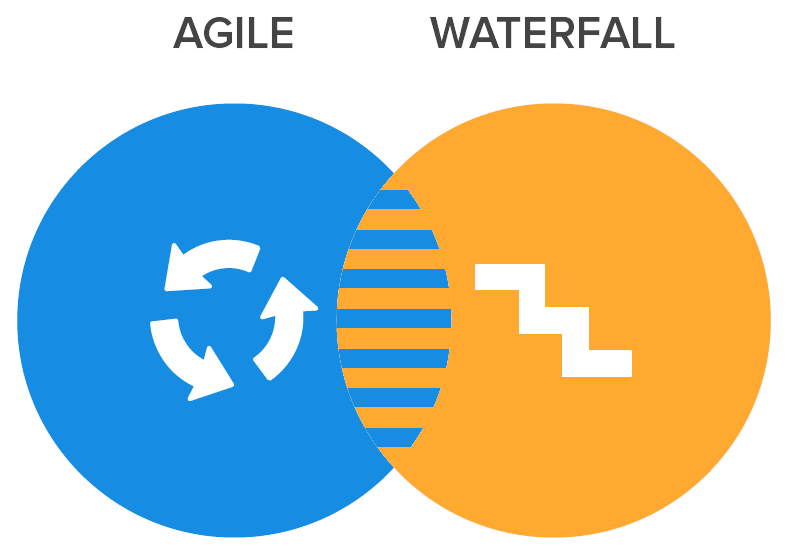
\includegraphics[width=0.4\textwidth]{figures/agile-waterfall}
    \caption{Balanced Approach to Waterfall and Agile Methodologies}
\end{figure}

In the context of my work, the approach is that prototypes, PoCs and internal beta versions of new software products are developed using various Agile Methodologies (Scrum and Kanban) and once their purpose is verified, the work done is considered as the starting point for the SDLC.

\section{Current Workflow}

Currently, the top management is in the USA, while the innovation department is in Prague, Czech Republic. Some members from the top management occasionally fly to Prague, but very irregularly and mostly for a quick check on the overall status of the department. Most of the communication happens remotely - via video conference calls, e-mails etc. Obviously, this produces a lot of noise in the data being transferred. Sometimes some parts are misheard or misunderstood, get lost and are causes for a larger problem in the future.

Not only there is a difference in the culture and language, but it clearly leads to a difference in the domain vocabularies used in everyday work. Tools for productive data exchange are implemented - such as:

\begin{itemize}
	\item Issue tracker
	\item Internal Wiki-style website
	\item Enterprise chat
\end{itemize}

But the problem is, that there is no tool that unites them all to make sure that the domain vocabularies are the same throughout the whole development phase. If such tool existed, a one that could connect to all of the deployed knowledge systems, it would make communication of measured performance of a product a lot easier.

Let's take a look at the current tools available on the market that specialize in application performance measuring.

\section{Existing Tools}

I will now analyze and assess the tools available on the market. I'll focus primarily on the flexibility of the deployment and their analysis features. Anything else has a minor priority.

\subsection{Google Analytics}

Google Analytics is by far the most popular and widely used framework for monitoring user interactions in applications. It reports everything the developer wishes to. By default it does not report anything - the tool has to be activated during application start. Then each action needs to be hard-coded in the code. An action can be two things - the first one is after a certain user activity has happened - a press of a button, pulling down a list to refresh the data etc. One thing gets reported - "this event has happened". The second one is more open - an identifier is set to an item, let's say, a button. Whatever happens with that button gets reported, be it touch, swipe or anything else.

\begin{figure}[!ht]
	\centering
	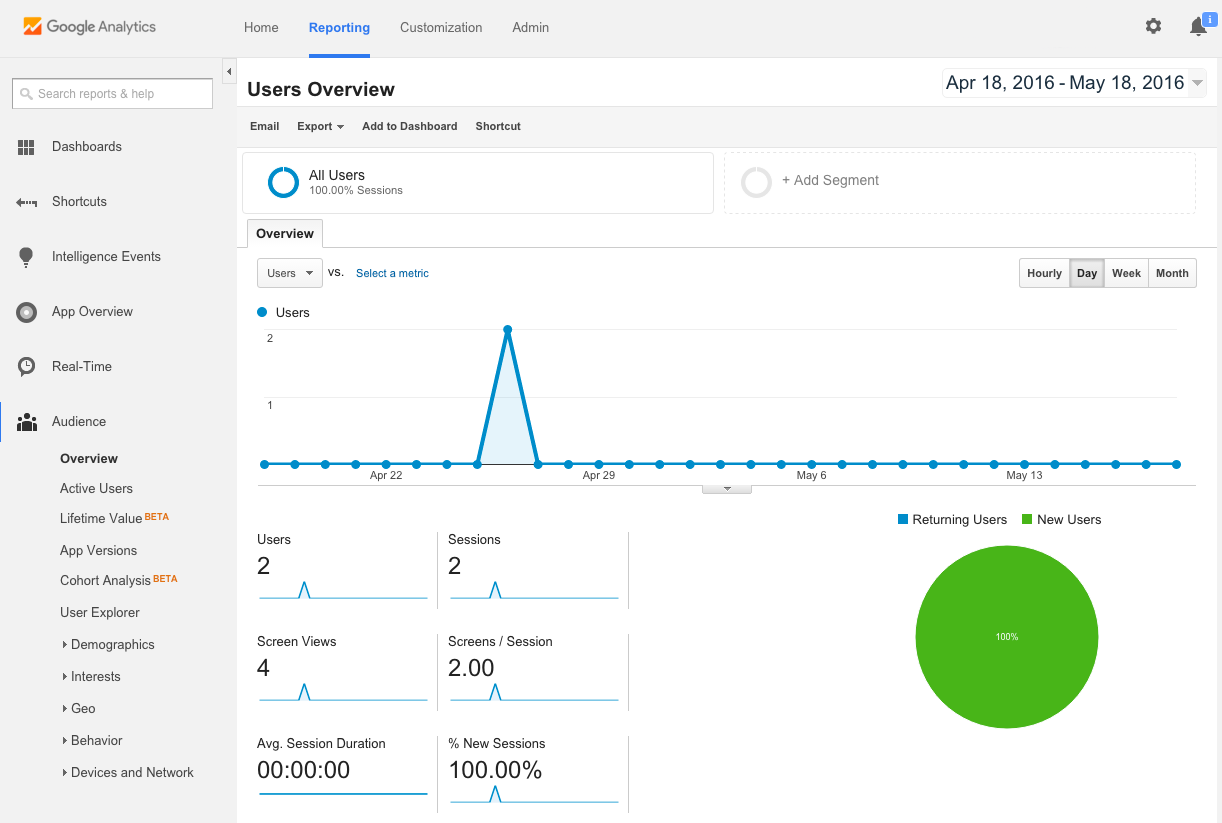
\includegraphics[width=0.65\textwidth]{figures/analytics}
    \caption{Google Analytics Dashboard}
\end{figure}

The dashboard website is very detailed and responsive. All data is nicely visualized in graphs and corresponds well with the whole GA ecosystem. Higher order semantics is remotely possible via definition of complex queries and dashboard setups. User management is very rich and enables forming multiple roles for different users. The main problem is, unfortunately, that all data goes to Google. There is no option of having the engine run on custom servers. All code is closed source and that simply wouldn't go through any risk assessments because Google might be sending the data to anywhere in the world.

Data is accessible via REST API, but registration for it is required (it is not possible for a "normal" user to start using the REST API). Single user account is free, enterprise account is paid.

\subsection{Google Tag Manager}

Google Tag Manager is a tag management system that allows quick and easy update of tags and code snippets in a mobile application. It allows adding and updating AdWords, Google Analytics, etc. from the Tag Manager user interface instead of editing the code.

A tag is a snippet of code that sends information to Google. It is not necessary to wire it up in code - it works through configuration files from the admin user interface.

Tag Manager is deployed in conjunction with the Firebase SDK, with support for both Android and iOS. The container replaces all other manually-coded tags in the mobile application, including tags from AdWords, Google Analytics etc. It basically builds on top of Google Analytics to make the integration a little easier. It is aimed to be used by people focused mainly on marketing, thus the tool itself serves as an overall performance dashboard. It allows them to create complex tags in a short period of time. Unfortunately it works well only on the web - the tags have to be hard-coded in mobile applications.

\newpage

\begin{figure}[!ht]
	\centering
	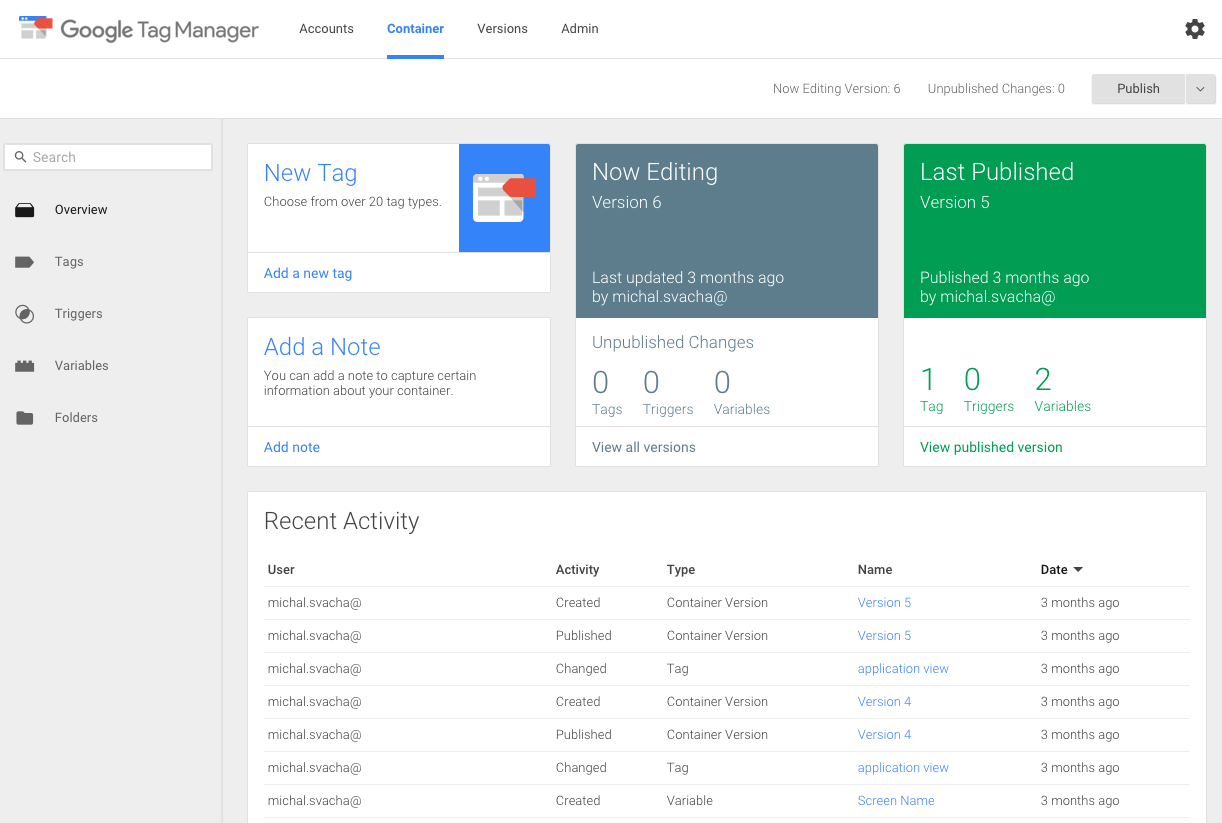
\includegraphics[width=0.65\textwidth]{figures/tagmanager}
    \caption{Google Tag Manager Dashboard}
\end{figure}

The dashboard is similar in style to the Google Analytics one. Tags can be created, modified and linked with a specific Google Analytics query. The same as for Google Analytics holds for Google Tag Manager - everything is closed source and runs exclusively on Google's servers.

\subsection{Tealium}

Tealium is a complex tool combining all marketing tools on the market (Criteo, Socialbakers, but also Google AdWords etc.). It does offer insights into usage and performance and it is very robust. 

\bigbreak

"Combining the leading enterprise tag management solution, an omnichannel customer segmentation and action engine, and a suite of rich data services, the Tealium CDP enables organizations to unlock customer data trapped in siloed marketing systems, build a unified customer view, and take real-time action." \cite{tealium}

\bigbreak

As of December 2015, Tealium successfully completed a Health Insurance Portability and Accountability Act (HIPAA) and Health Information Technology for Economic and Clinical Health Act (HITECH) attestation examination \cite{hipaa}, making it compliant to store data in the cloud securely. The only limitation with this is, that it is only valid in the USA - it does not extend to countries such as China, Japan or Russia, where customer data have to be stored within the country's borders.

The tool itself is intended to be wired up and used as-is. Tealium has their own servers, their won front-end and no API. While for smaller to mid-sized companies it may be sufficient, larger companies require code customizations and integrations into their systems that are currently not provided by this tool.

\subsection{Fabric (formerly Crashlytics)}

Fabric is a platform made by Twitter. Collected and fine-tuned I should say, as it comprises of multiple acquired start-up platforms. The focal point of this platform is a former crash reporting tool Crashlytics \cite{crashlytics}. Aside from that Fabric is a full-featured developer platform used for a variety of tasks. It helps to overcome obstacles a developer may face - even the distribution of beta versions to testers, which has always been a problem for iOS developers.

\bigbreak

"The Fabric platform is made of three modular kits that address some of the most common and pervasive challenges that all app developers face: stability, distribution, revenue and identity. It combines the services of Crashlytics, MoPub,Twitter and others to help build more stable apps, generate revenue through the world’s largest mobile ad exchange and enable to tap into Twitter’s sign-in systems and rich streams of real-time content for greater distribution and simpler identity. Installation takes minutes, and most features only require a few lines of code." \cite{fabric}

\bigbreak

Fabric has been taken it a step further and is not only about reporting crashes, but it also reports overall statistics, like Google. One really nice feature is a video visualization of user movements in the application. Formerly Appsee \cite{appsee}, now a UX part of Fabric, creates a video of steps users take in the application to give the developer a new perspective on how their application is actually used.

The source code of Fabric is closed source (except for some parts, like Fastlane \cite{fastlane}) and all of the statistics run on Twitter's servers. The Data is not accessible in any other way, than via Fabric's custom dashboards. 

The whole platform is free to use. Registration of developers and applications is required along with the installation of a custom Fabric installation program which integrates the framework into existing projects.

\subsection{App Pulse (formerly Pronq)}

Hewlett-Packard Enterprise AppPulse Mobile is a mobile app performance monitoring tool that tracks the real user experience of mobile applications.

App Pulse is very different from the previously listed tools in a way that it reports everything at all times. The usage is fairly low - tens of kilobytes per week, but it is very thorough. Screen time, actions, movements - it is all there in the report and no setup is required for the start. That obviously leads to gathering a lot of junk by default.

Contrary to iOS standards, App Pulse's SDK is distributed via a compiled library that has to be drag-and-dropped manually into the Xcode project. This is not a good practice, as Apple's updates are regular and oftentimes break a lot of old code, so keeping the SDK up to date manually is a lot of pain.

Because it works out-of-the-box and "automagically" tracks everything that happen in the application, the one big issue is the need to have a consistent naming of all views, labels, buttons etc. - as it does everything on its own, without hooking up the actionable items to the framework manually, it can be hard to determine which button was referred to in the report. One really interesting feature is battery level monitoring, though it is disputable, as the user may have multiple applications running in the background.

Free 30-day trial allows up to two mobile applications, 25.000 active users per application (everything above is discarded, or offered for the standard monthly price) and access to the App Pulse community. The tools are closed source and all of the statistics runs on Hewlett-Packard Enterprise servers as it is a Software as a Service (= SaaS). No API is provided.

\subsection{Apteligent (previously Crittercism)}

Apteligent doesn't stand out from previously mentioned tools - it runs on Apteligent's own servers, has custom SDK and works seemlessly. While it does have some benchmarking that others don't, at the end of the day, Apteligent again is the owner of your users' data. It seems very enterprise oriented - it enables 3rd party API integration into their system, which enables monitoring the performance of other APIs used in the application to really find what can be the bottleneck of the overall performance.

The tools are closed source and all of the statistics run on Apteligent's servers. API for data retrieval is provided.

\subsection{New Relic}

Other than the standard package (SDK, custom servers, periodical reports), New Relic has a nice alerting system - when a crash occurs, a web hook to ticketing system can be defined to streamline bug reports into the issue tracker.

Similar to Tealium, New Relic does stand out with the focus on data encryption:

\bigbreak

"You have complete control over what, if any, sensitive information is sent to New Relic. We are unique among software analytics solutions. When you deploy our agent, by default, our security settings and regulatory compliance exceed industry standards, and all data is encrypted in transit." \cite{newrelic}

\bigbreak

While this is a good start, it simply isn't compliant with the legislation of many countries, to store the users' data on a "random" cloud computer storage. The iOS SDK is distributed in a compiled binary file, having enormous 28,5MB. It is not open sourced. API for data retrieval is provided.

\subsection{Apple}

The last tool I will mention isn't considered as a framework, but is important nonetheless. As companies fight for user data from mobile applications - such as Twitter, who even gives out their platform to everybody for free, naturally the platform owners (Apple and Google) strive for keeping all that precious data for themselves. Apple announced in 2015 at their Wordwide Developer Conference (= WWDC) a new iTunes Connect portal with a new feature - App Analytics. 

\newpage

\begin{figure}[!ht]
	\centering
	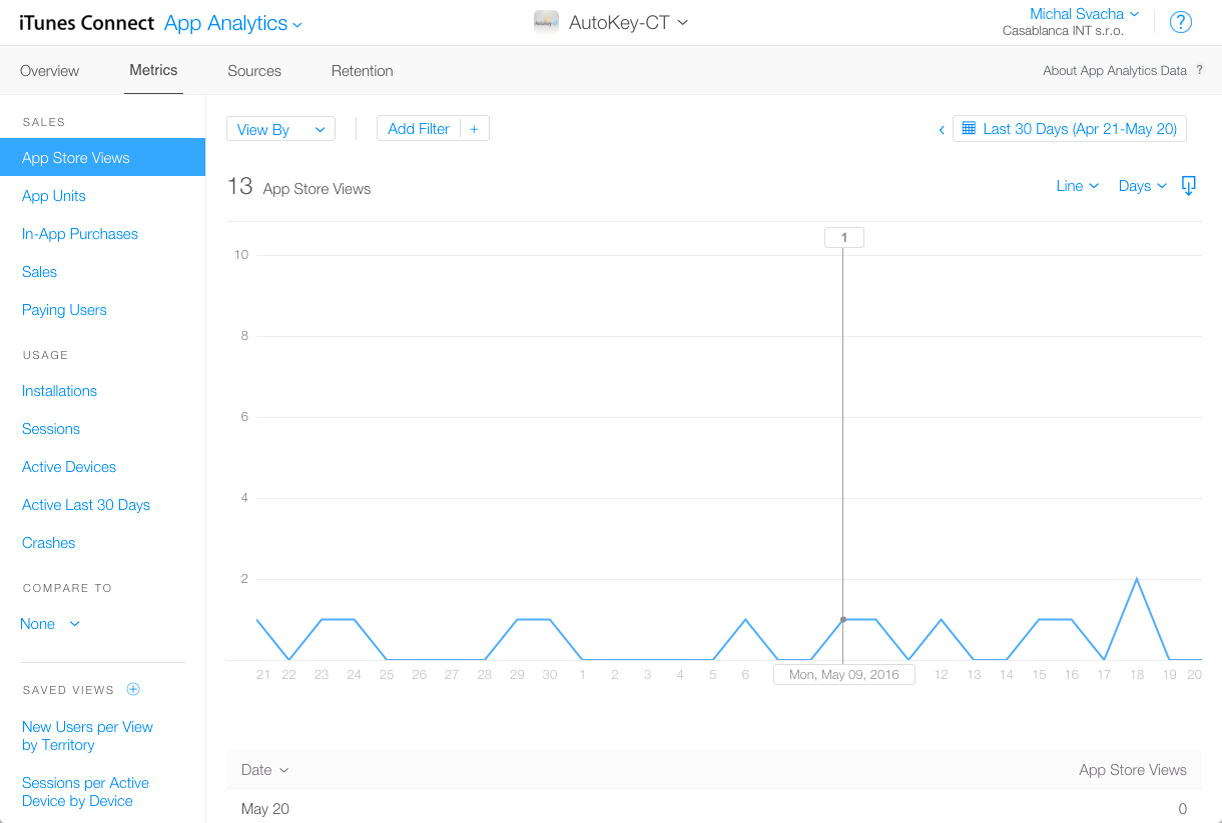
\includegraphics[width=0.65\textwidth]{figures/appleanalytics}
    \caption{Apple App Analytics Dashboard}
\end{figure}

It is fairly thorough in means of usage, downloads, screen time etc., but the overall reporting seems very marketing oriented. Crashes do get reported, but not they are not very detailed compared to Fabric's Crashlytics tool.

One of the biggest obstacles every iOS developer faces is the fact that since iOS 5 \cite{udid} it is not possible to uniquely identify a device. Therefore it is virtually impossible to connect two user entries of the same user if the user deletes and redownloads the application. The only way it could be identified is through Apple's own analytics solution. However, the help tooltip for Installations says:

\bigbreak

"The total number of app installations and redownloads. Installations doesn't include app updates."

\bigbreak

Which looks like Apple disabled identification of the same device for themselves as well. 

App Analytics in iTunes Connect is provided to every single developer automatically for free on the iTunes Connect website. There is no framework to be implemented, the statistics is gathered whether the developer likes it or not. Naturally Apple keeps all of the user data on their servers. Even though iTunes Connect has a JSON REST API, none of the sales or analytics data endpoints are exposed.

\newpage

\section{Conclusion on tools}

\begin{enumerate}
	\item Google Analytics
		\begin{itemize}
			\item[{\bf PROS:}] robustness, reliability, reputation
			\item[{\bf CONS:}] completely proprietary, very low-level
		\end{itemize}
	\item Google Tag Manager
		\begin{itemize}
			\item[{\bf PROS:}] abstraction above GA, flexibility
			\item[{\bf CONS:}] completely proprietary, hard initial setup
		\end{itemize}
	\item Tealium
		\begin{itemize}
			\item[{\bf PROS:}] versatility, omni-channel connectivity
			\item[{\bf CONS:}] completely proprietary
		\end{itemize}
	\item Fabric
		\begin{itemize}
			\item[{\bf PROS:}] versatility, community support
			\item[{\bf CONS:}] completely proprietary, required Twitter registration, data inaccessibility
		\end{itemize}
	\item App Pulse
		\begin{itemize}
			\item[{\bf PROS:}] automatic initial setup
			\item[{\bf CONS:}] completely proprietary, non-standard SDK distribution, data inaccessibility
		\end{itemize}
	\item Apteligent
		\begin{itemize}
			\item[{\bf PROS:}] 3rd party tool integration
			\item[{\bf CONS:}] completely proprietary
		\end{itemize}
	\item New Relic
		\begin{itemize}
			\item[{\bf PROS:}] user data encryption
			\item[{\bf CONS:}] completely proprietary, non-standard SDK distribution
		\end{itemize}
	\item Apple
		\begin{itemize}
			\item[{\bf PROS:}] no installation or setup required
			\item[{\bf CONS:}] completely proprietary, data inaccessibility
		\end{itemize}
\end{enumerate}

None of the tools meet the requirements for deployment (custom servers) and therefore privacy as well for a global enterprise in regulated market. It is necessary to design an architecture that would fit the needs - run the whole solution on custom servers and enable the mash-up of various knowledge resources deployed across the company.